\chapter{Metodología}\label{cap:3}
\lettrine{P}{ara modelar el proceso de amplificación} de la semilla de armónicos de alto orden introducida a través del canal de plasma, es necesario plantear y resolver numéricamente las denominadas en la literatura como ecuaciones de Maxwell-Bloch o \emph{\acrfull{mbe}}. El código Dagon empleado durante las simulaciones implementa estas ecuaciones mediante un programa escrito en Fortran que, a su vez, está acoplado con otros códigos numéricos ---cuya función se explicará más detalladamente en la sección \S\ref{sec:3.2}---, recibiendo información de partida para iniciar el procedimiento de cálculo. De esta forma, los resultados proporcionan los datos necesarios para comprender cómo afectan la densidad de iones y electrones libres en el plasma a la intensidad y perfil de fase del haz \acrshort{xuv} obtenido. 

Una vez finalizadas las simulaciones, para poder realizar el análisis de las imágenes y los resultados obtenidos, se emplearon dos nuevos programas ---esta vez escritos en Python y Octave---, que permiten almacenar los datos obtenidos en las simulaciones de Dagon y representarlos gráficamente mediante curvas bidimensionales. Además, estos conjuntos de datos pueden introducirse en programas como VisIt para la construcción de imágenes tridimensionales y bidimensionales, por ejemplo, de la propagación del \acrshort{hoh} en la dirección longitudinal del canal.

\section{Ecuaciones de Maxwell-Bloch}\label{sec:3.1}
En este trabajo, el fenómeno físico de la amplificación del armónico inyectado en el plasma de iones de kriptón conduce inevitablemente hasta estas ecuaciones, puesto que determinan cuáles serán las propiedades de la emisión obtenida. Las \acrshort{mbe} describen la dinámica de la interacción entre los modos de vibración de un campo electromagnético y los átomos de un sistema cuántico con dos estados posibles $\ket{1}$ y $\ket{2}$. 

El formalismo físico-matemático utilizado en mecánica cuántica para obtener las ecuaciones no es trivial\autocite{Cohen-Tannoudji2019a,Sakurai2020,Milonni1988}, aunque tiene la ventaja de predecir con suficiente exactitud la evolución temporal del pulso, además de propiedades físicas de los fotones como su \acrshort{oam}, mientras que otros métodos más sencillos ---como el programa de trazado de rayos SHADOX--- no ofrecen esta opción, si bien podría utilizarse para resolver el problema de la amplificación en el plasma. 

En la interacción láser-plasma estudiada, para obtener una buena aproximación basta considerar el campo eléctrico $\symbfcal{E}$ de la semilla \acrshort{hoh}, aunque cálculos más precisos tendrían que incorporar el acoplamiento del campo magnético $\symbfcal{B}$. Además, el acoplamiento entre el campo electromagnético y la materia utiliza una aproximación semiclásica, donde los átomos o iones son sistemas cuánticos de dos estados descritos por la ecuación de Schrödinger, mientras que la luz es un sistema clásico ---una onda electromagnética--- descrito por las ecuaciones de Maxwell.

En primer lugar, el acoplamiento del campo eléctrico con el plasma es la ecuación de ondas 
\begin{equation}\label{eq:3.1}
  \laplacian \symbfcal{E} - \frac{1}{c^{2}}\pdvN{\symbfcal{E}}{t}{2} = \frac{\omega^{2}_{pe}}{c^{2}}\symbfcal{E} + \frac{1}{\epsilon_{0}c^{2}}\pdvN{\symbfcal{P}}{t}{2},
\end{equation}
donde el campo eléctrico $\symbfcal{E}$, la polarización $\symbfcal{P}$, la frecuencia de las oscilaciones del plasma $\omega_{pe}$ y la constante dieléctrica $\epsilon_{0}$ son función del espacio y del tiempo, mostrado en la sección \S\ref{sec:1.2.2}. 

Como primera hipótesis, se considera la llamada en óptica\autocite{Born2019} como \emph{aproximación paraxial} del campo eléctrico según la dirección de propagación escogida, en este caso, el eje $z$. Suponiendo que la radiación está polarizada linealmente según el eje $x$, esta simplificación permite tener en cuenta únicamente la componente $x$ del campo eléctrico y de la polarización, dirección en la que oscilarían ambos campos, escribiendo por separado la envolvente y las vibraciones del mismo como
\begin{align}
  \label{eq:3.2a}
  \symcal{E}_{x}(\symbf{r},t) &= \RE \left[E_{+}(\symbf{r},t)\eu^{\iu (kz - \omega t)} + E_{-}(\symbf{r},t)\eu^{\iu (kz + \omega t)}\right], \\
  \label{eq:3.2b}
  \symcal{P}_{x}(\symbf{r},t) &= \RE \left[P_{+}(\symbf{r},t)\eu^{\iu (kz - \omega t)} + P_{-}(\symbf{r},t)\eu^{\iu (kz + \omega t)}\right], 
\end{align}
donde $E_{+}$, $E_{-}$, $P_{+}$, $P_{-}$ son la amplitud de las oscilaciones de las ondas viajeras hacia la dirección positiva y negativa del eje $z$, respectivamente, es decir, las envolventes. 

Combinando las ecuaciones \eqref{eq:3.1} y \eqref{eq:3.2a}, y agrupando las componentes que se propagan a lo largo de todo el eje $z$, se obtiene para el campo eléctrico
\begin{align}
  \laplacian \symcal{E}_{x} 
  &= 
  \RE \Bigg[\left(\pdvN{E_{\pm }}{x}{2} + \pdvN{E_{\pm }}{y}{2} + \pdvN{E_{\pm }}{z}{2} + 2k \iu \pdv{E_{\pm }}{z} - k^{2}E_{\pm }\right)\eu^{\iu (kz \mp \omega t)}\Bigg], \\
  \pdvN{\symcal{E}_{x}}{t}{2}
  &= 
  \RE \Bigg[\left(\pdvN{E_{\pm }}{t}{2} \mp 2 \omega \iu \pdv{E_{\pm }}{t} - \omega^{2}E_{\pm }\right)\eu^{\iu (kz \mp \omega t)}\Bigg],
\end{align}
obteniéndose el lado izquierdo ($\mathrm{LHS}$) de la ecuación de ondas para el campo eléctrico
\begin{equation}\label{eq:3.3}
  \begin{split}
    \mathrm{LHS} = \RE \Bigg[\bigg(\laplacian_{\perp}E_{\pm} &+ \pdvN{E_{\pm }}{z}{2} + 2k \iu \pdv{E_{\pm }}{z} - \frac{1}{c^{2}}\bigg(\pdvN{E_{\pm }}{t}{2} \pm 2 \omega \iu \pdv{E_{\pm }}{z}\bigg) \\ &+  \bigg(\frac{\omega^{2}}{c^{2}} - k^{2}\bigg)E_{\pm }\bigg)\eu^{\iu(kz \mp \omega t)}\Bigg],
  \end{split}
\end{equation}
donde $\laplacian_{\perp}$ es el operador laplaciano transversal sobre el plano $xy$, definido como
\begin{equation*}
    \laplacian_{\perp} \equiv \pdvN{E_{\pm }}{x}{2} + \pdvN{E_{\pm }}{y}{2}.
\end{equation*}
La ecuación \eqref{eq:3.3} puede reducirse más simplificando la relación de dispersión del campo eléctrico en el plasma $\omega^{2} = \omega^{2}_{pe} + k^{2}c^{2}\approx k^{2}c^{2}$, puesto que para la emisión de radiación \acrshort{xuv} o rayos X blandos ($\lambda<\qty{40}{nm}$) y la densidad electrónica del plasma de kriptón ($n_e<\qty{e21}{cm^{-3}}$) se tiene que, por un lado, $\omega_{pe}<\qty{1,8e15}{rad/s}$ y, por otra parte, $\omega>\qty{4,7e16}{rad/s}$, luego necesariamente $\omega>\omega_{pe}$ y la aproximación de la relación de dispersión estaría justificada, ya que ambos términos difieren como mínimo en dos órdenes de magnitud. 

Continuando nuevamente con las hipótesis, es importante considerar la aproximación de la envolvente lentamente variable o \emph{\acrfull{svea}} que asume la variación temporal y espacial de la envolvente $F$ lenta\autocite{Larroche2000} comparada con su longitud de onda, de manera que ambas envolventes del campo eléctrico y polarización verifican
\begin{equation}\label{eq:3.4}
  \abs{\pdvN{F}{z}{2}} \ll \abs{k \pdv{F}{z}} \ll \abs{k^{2} F}, \quad 
  \abs{\pdvN{F}{t}{2}} \ll \abs{\omega \pdv{F}{t}} \ll \abs{\omega^{2} F}.
\end{equation}

Para señalar la importancia del concepto de la \acrshort{svea} en la resolución de las \acrshort{mbe} mediante cualquier método numérico, la Figura \ref{fig:3.1} muestra esquemáticamente un pulso cuya envolvente ---del campo eléctrico--- varía lentamente, propagándose en la dirección $z$.
\begin{figure}[ht!]
  \centering
  \begin{subcaptionblock}{.4\textwidth}
    \centering
    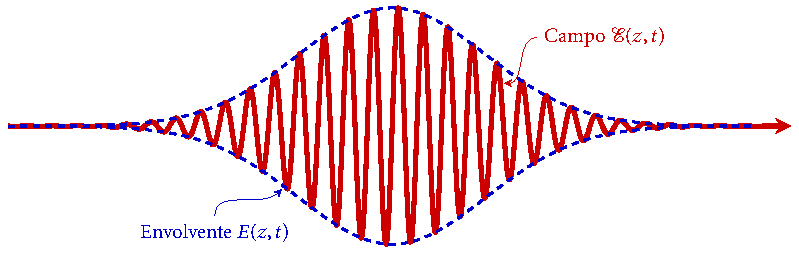
\includegraphics[width=1.2\textwidth]{Figuras/ch3_pulso2d.pdf}
    \caption{Pulso 2D}\label{fig:3.1a}
  \end{subcaptionblock}%
  \begin{subcaptionblock}{.4\textwidth}
    \centering
    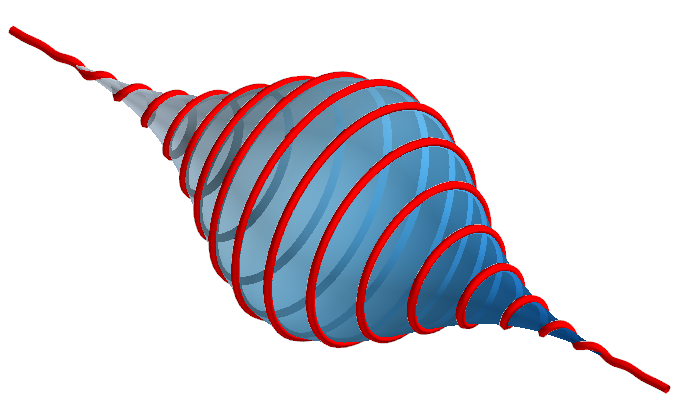
\includegraphics[width=0.8\textwidth]{Figuras/ch3_pulso3d.png}
    \caption{Pulso 3D}\label{fig:3.1b}
  \end{subcaptionblock}%
  \caption{Representación 2D y 3D de un pulso láser con la aproximación \acrshort{svea}.}
  \label{fig:3.1}
\end{figure}

A modo ilustrativo, la Figura \ref{fig:3.1b} del pulso tridimensional ha sido elaborada mediante la escritura del Código \ref{cod:3.1} que recurre a la librería Mayavi de Python para su representación.
\begin{listing}[htbp!]
  \caption{Código escrito para representar una \acrshort{svea} de un pulso 3D.}
  \inputminted[firstline=8, lastline=40]{python}{Programas/mlaser.py}
  \label{cod:3.1}
\end{listing}

Empleando las aproximaciones para la relación de dispersión y la envolvente del campo eléctrico consideradas, la ecuación \eqref{eq:3.3} finalmente queda
\begin{equation}\label{eq:3.5}
  \mathrm{LHS} =
  \RE \Bigg[\left(\laplacian_{\perp}E_{\pm } + \frac{2 \omega \iu }{c^{2}} \left(\pdv{E_{\pm }}{t} \pm c \pdv{E_{\pm }}{z}\right)\right)\eu^{\iu (kz \mp \omega t)}\Bigg].
\end{equation}

En segundo lugar, el lado derecho ($\symrm{RHS}$) de la ecuación \eqref{eq:3.1} contiene el término para la polarización del plasma, cuya descomposición en ondas viajeras mostraba la ecuación \eqref{eq:3.2b}, obteniéndose que
\begin{equation}\label{eq:3.6}
  \pdvN{\symcal{P}_{x}}{t}{2} = 
  \RE \Bigg[\left(\pdvN{P_{\pm }}{t}{2} \mp 2 \omega \iu \pdv{P_{\pm }}{z} - \omega^{2}P_{\pm }\right)\eu^{\iu (kz \mp \omega t)}\Bigg].
\end{equation}
Recordando la aproximación \acrshort{svea} de la ecuación \eqref{eq:3.4} para las envolventes junto a la relación de dispersión $\omega^{2} \approx k^{2}c^{2}$, puede considerarse que la amplitud de la polarización en un periodo de onda $\omega$ es mucho mayor que la variación temporal de su envolvente, es decir,
\begin{equation}
  \abs{\pdv{P_{\pm }}{t}} \ll \abs{\omega P_{\pm }},
\end{equation}
quedando la ecuación \eqref{eq:3.6} como
\begin{equation}\label{eq:3.7}
  \pdvN{\symcal{P}_{x}}{t}{2} = \RE \left[- \omega^{2}P_{\pm }\eu^{\iu (\omega t \pm kz)}\right].
\end{equation}
Por último, la sustitución de las ecuaciones \eqref{eq:3.5} y \eqref{eq:3.7} en la ecuación \eqref{eq:3.1} permite obtener, tras reagrupar los términos a izquierda ($\symrm{LHS}$) y derecha ($\symrm{RHS}$), respectivamente
\begin{equation}\label{eq:3.8}
  \pdv{E_{\pm }}{t} \pm c \pdv{E_{\pm }}{z} = \frac{\iu c^{2}}{2 \omega}\laplacian_{\perp}E_{\pm } + \frac{\iu \omega}{2} \left[\mu_{0}c^{2}P_{\pm } - \left(\frac{\omega_{pe}}{\omega}\right)^{2}E_{\pm }\right],
\end{equation}
obteniendo una ecuación en derivadas parciales de segundo orden en el espacio y primer orden en el tiempo con un término fuente $P_{\pm}$ función de las coordenadas espaciales y temporales. Adicionalmente, haciendo un cambio de variable $\xi = c \tau$, y definiendo un \enquote{tiempo reducido} como $\tau = t \pm z/c$, la ecuación \eqref{eq:3.8} puede escribirse 
\begin{equation}
  \pdv{E_{\pm }}{\xi} = \frac{\iu c}{2 \omega}\laplacian_{\perp}E_{\pm } + \frac{\iu \omega}{2c} \left[\mu_{0}c^{2}P_{\pm } - \left(\frac{\omega_{pe}}{\omega}\right)^{2}E_{\pm }\right],
\end{equation}
aunque esta transformación sería especialmente útil en el esquema unidimensional, donde el primer sumando del lado derecho ($\symrm{RHS}$) es nulo, pues el plano $xy$ desaparecería del problema.

Hasta este momento, el marco teórico utilizado para el tratamiento de la radiación ha sido clásico, pero como se ha explicado al principio de este sección \S\ref{sec:3.1}, la teoría electromagnética clásica no proporciona una descripción satisfactoria \autocite{Griffiths2017} de la interacción entre la luz y la materia a estas escalas, siendo necesario cuantizar el comportamiento de la materia para comprender la polarización resultante.

Por tanto, hay que introducir una ecuación constitutiva que relacione la naturaleza de la interacción entre la luz (el campo eléctrico), y la materia (la polarización). En la teoría cuántica, la relación \autocite{Cohen-Tannoudji2019} viene dada por
\begin{equation}\label{eq:3.9}
  \xval{P} = \symrm{Tr} \left(\rho \symcal{D} \right),
\end{equation}
donde $\rho$ es el operador de densidad, $\symcal{D}$ el operador momento dipolar eléctrico atómico y $\symrm{Tr}$ representa la traza (suma de los elementos de la diagonal principal) del producto de ambos operadores, expresados como matrices en una base ortonormal $\left\{\ket{u_{i}(\symbf{r})}\right\}_{i \in \symbb{N}} \in \symcal{F}$, siendo $\symcal{F}$ un subespacio vectorial \autocite{Cohen-Tannoudji2019} formado por funciones suficientemente regulares para estudiar este fenómeno. Empleando como base los estados $\ket{1}$ y $\ket{2}$ del sistema (que están normalizados a la unidad), la matriz de densidad es
\begin{equation}\label{eq:3.10}
  \rho(\symbf{r},t) = 
  \begin{pmatrix}
    \rho_{11}(\symbf{r},t) & \rho_{12}(\symbf{r},t) \\
    \rho_{21}(\symbf{r},t) & \rho_{22}(\symbf{r},t)
  \end{pmatrix}.
\end{equation}

Con el objetivo de aportar mayor claridad en la discusión cuántica de la polarización, es necesario realizar una breve explicación de los conceptos introducidos y su significado. El plasma objeto de estudio puede aproximarse \autocite{Milonni1988} como un sistema de dos estados $\ket{1}$ y $\ket{2}$ posibles linealmente independientes \autocite{Cohen-Tannoudji2019}, de manera que la probabilidad de encontrarse en cualquiera de ambos estados es $p_{1} + p_{2} = 1$.

En este contexto, el momento dipolar eléctrico $\symcal{D}$ es el observable que se desea medir, y la polarización $\xval{P}$ es el valor esperado. El operador de densidad es particularmente importante en sistemas donde no se conoce (o es imposible conocer) la totalidad de la información sobre el estado inicial del sistema ---los iones y electrones del plasma en este caso---, ni tampoco pueden determinarse con total precisión los resultados de las mediciones debido a la naturaleza probabilística de los sistemas cuánticos. 

Ambos estados, pertenecientes al espacio vectorial $\symcal{F}$, pueden emplearse como una base ortonormal, pues como se ha comentado anteriormente, son linealmente independientes y están normalizados a la unidad, de tal forma que en el caso más general posible, el estado del sistema puede ponerse como combinación lineal de ambos
\begin{align}
  \ket{\psi} = c_{1}\ket{1} + c_{2}\ket{2} &= \sum_{k} c_{k}\ket{k}, \\
  \abs{c_{1}}^{2} + \abs{c_{2}}^{2} &= 1,
\end{align}
con $k \in \{1,2\}$ un subíndice para designar cualquiera de los dos estados posibles. La superposición de ambos estados implica que los elementos $\rho_{nn}$ y $\rho_{nm}$ de la matriz de densidad pueden escribirse como
\begin{equation}\label{eq:3.11}
  \rho_{nn} = \abs{c_{n}}^{2}, \quad 
  \rho_{nm} = c_{n}c^{*}_{m}
\end{equation}
donde $\abs{c_{n}}^{2}$ es un número real positivo que representa la probabilidad, en una medición del sistema en el estado superpuesto $\ket{\psi}$, de encontrarlo en el estado $\ket{n}$. Por otro lado, los términos cruzados de la forma $c_{n}c^{*}_{m}$ expresan el fenómeno de interferencia que puede aparecer entre dos estados $\ket{n}$ y $\ket{m}$ cuando el estado $\ket{\psi}$ es una superposición lineal de los anteriores, como ocurre en este modelo. 

Observando la ecuación \eqref{eq:3.11}, está claro que $\rho_{nn}$ es cero solamente si los $c_{n}$ son cero, mientras que $\rho_{nm}$ puede ser cero cuando alguno (o los dos) de los términos cruzados $c_{n}$ o $c^{*}_{m}$ son cero, siendo estos números complejos. Por lo tanto, si $\rho_{nm}$ es cero significa que los efectos de interferencia entre los estados $\ket{n}$ y $\ket{m}$ han desaparecido, mientras que si $\rho_{nm}$ es distinto de cero entonces persiste una cierta \enquote{coherencia} entre ambos estados, motivo por el cual los elementos fuera de la diagonal $\rho_{nm}$ son llamados \emph{coherencias}.

A raíz de esta exposición, las entradas de la matriz de densidad tienen el siguiente significado: los elementos en la diagonal principal $\rho_{nn}$ representan la probabilidad media de encontrar el sistema en el estado $\ket{n}$, motivo por el que se conocen como las \emph{poblaciones} del estado $\ket{n}$, ya que para un número elevado $N$ de mediciones de la misma propiedad, bajo las mismas condiciones iniciales, $N \rho_{nn}$ sistemas estarán en el estado $\ket{n}$. En cambio, $\rho_{nm}$ es la coherencia entre los dos niveles atómicos del plasma, luego está relacionado con la capacidad del campo eléctrico $\symcal{E}$ del \acrshort{hoh} de provocar la polarización de las partículas que lo constituyen.

Es posible demostrar \autocite{Cohen-Tannoudji2019} que el conocimiento de la matriz de densidad es suficiente para caracterizar el sistema cuántico, empleando la ecuación de Schrödinger (Bloch)
\begin{equation}\label{eq:3.12}
  i \hslash \pdv{\rho(\symbf{r},t)}{t} = \left[H(\symbf{r},t),\rho(\symbf{r},t)\right],
\end{equation}
con $H = H_{O} + V_{DE}(\symbf{r},t)$, siendo $H_{O}$ el operador Hamiltoniano atómico, $V_{DE} = -\symcal{D} \cdot E(\symbf{r},t)$ el potencial electrostático que encierra la interacción entre el campo eléctrico y los estados del sistema, y $\left[H, \rho\right] = H \rho - \rho H$ el conmutador de ambos operadores. Esta expansión del Hamiltoniano es conocida como \emph{aproximación dipolar} \autocite{Jackson1998} y es válida cuando la longitud de onda de la radiación emitida ---rayos X blandos en este caso--- es considerablemente superior que el tamaño promedio del átomo estudiado ($\lambda \sim \qty{10}{nm}$ frente a $R_{a} \sim \qty{0.1}{nm}$ de radio atómico). 

Realmente, el operador momento dipolar eléctrico $\symcal{D}$ puede escribirse como $\symcal{D} = -e \hat{r}_{a}$, siendo $\hat{r}_{a}$ el operador posición relativa entre el núcleo atómico y el electrón, y $e$ la carga eléctrica del electrón. Esto significa que puede representarse como un vector cuyos componentes son los elementos fuera de la diagonal principal de la matriz dipolar asociada, ya que $\symcal{D}$ representa el momento dipolar eléctrico asociado a la transición entre estados ---que naturalmente son diferentes---, y por tanto, los elementos de la diagonal principal tienen que ser cero. Debido a esto, el potencial de interacción puede ponerse como
\begin{equation}
  V_{DE}(\symbf{r},t) = -\symcal{D} \cdot E(\symbf{r},t) =  
  \begin{pmatrix}
    0 & d_{12}E(\symbf{r},t) \\
    d_{21}E(\symbf{r},t) & 0 \\
  \end{pmatrix},
\end{equation}
con los elementos del momento dipolar eléctrico calculados mediante el producto escalar 
\begin{equation}\label{eq:3.13}
  d_{nm} = \bra{n}d \ket{m} = -e \int \varphi^{*}_{n}(\hat{\symbf{r}_{a}}) \hat{\symbf{r}_{a}} \varphi_{m}(\hat{\symbf{r}_{a}}) \diff^{3}\hat{r}_{a},
\end{equation}
siendo $\varphi_{n}(\hat{\symbf{r}_{a}})$ y $\varphi_{m}(\hat{\symbf{r}_{a}})$ las funciones de onda asociadas a los estados $\ket{n}$ y $\ket{m}$, con $n, m \in \{1,2\}$ los únicos dos posibles estados atómicos del plasma.

Regresando a la obtención de la matriz de densidad descrita por la ecuación \eqref{eq:3.12}, despreciando los efectos de interferencia debidos al efecto Zeeman \autocite{Sureau1995} y suponiendo que el tiempo característico de expansión hidrodinámica del plasma es mucho mayor que el de evolución de la polarización, sus términos no diagonales pueden obtenerse a partir de las conocidas en mecánica cuántica \autocite{Milonni1988} como ecuaciones ópticas de Bloch o \emph{\acrfull{obe}}
\begin{align}
  \label{eq:3.14a}
  \pdv{\rho_{21}}{t} &= -\gamma \rho_{21} - \frac{id_{21}}{\hslash }E_{\pm }\left(N_{2}-N_{1}\right), \\
  \label{eq:3.14b}
  \pdv{\rho_{12}}{t} &= -\gamma \rho_{12} + \frac{id_{12}}{\hslash }E_{\pm }\left(N_{2}-N_{1}\right),
\end{align}
donde $\gamma$ es la tasa de despolarización debida a los choques entre los iones y los electrones libres del plasma, otorgando información acerca de los intervalos de tiempo donde hay pérdida de polarización en el medio, y los términos $N_{2}$, $N_{1}$ representan las poblaciones de los dos estados atómicos, es decir, los elementos diagonales de la matriz de densidad. Además, también es posible encontrar otra relación mediante la cuantización del campo electromagnético \autocite{Cohen-Tannoudji2019b} ---fuera completamente del alcance de esta exposición---, entre el coeficiente de Einstein $A_{21}$ para la emisión espontánea, presentada en la sección \S\ref{sec:1.1.1}, y los términos de la matriz dipolar eléctrica, tal que 
\begin{equation}\label{eq:3.15}
  d_{21} = \sqrt{3 \pi A_{21} \hslash c^{3} \epsilon_{0}\omega^{-3}_{0}}, 
\end{equation}
donde es importante observar, a partir de las ecuaciones \eqref{eq:3.13}, \eqref{eq:3.14a} y \eqref{eq:3.14b}, que $\rho_{nm} = \rho^{*}_{mn}$ y, entonces, teniendo en cuenta que el operador $\symcal{D}$ es hermítico, $d_{nm} = d^{*}_{mn}$. De este forma, empleando la ecuación \eqref{eq:3.15} pueden determinarse los dos términos de la matriz dipolar.
Para terminar, combinando las ecuaciones \eqref{eq:3.8}, \eqref{eq:3.14a} y \eqref{eq:3.14b} se obtiene 
\begin{equation}\label{eq:3.16}
  \pdv{P_{\pm }}{t} = \Gamma - \gamma P_{\pm } + \frac{\iu \left(d^{2}_{12} + d^{2}_{21}\right)}{\hslash }E_{\pm }\left(N_{2}-N_{1}\right),
\end{equation}
donde $\Gamma$ es un término fuente introducido \autocite{Oliva2012} para modelar el comportamiento estocástico de la emisión espontánea, que incorpora el perfil Lorentziano de la línea de emisión del láser empleado mediante una función correlación de desvanecimiento. Las poblaciones podrían calcularse a través de las \acrshort{obe} restantes ---no incluidas anteriormente--- o, empleando el método utilizado en Dagon, a partir de las ecuaciones de tasas acopladas 
\begin{equation}\label{eq:3.17}
  \pdv{N_{k}}{t} = \sum_{i} C_{ik}N_{i} \pm \frac{1}{2 \hslash }\IM \left(E_{\pm }^{*}P_{\pm }\right),
\end{equation}
donde el sumatorio recorre todos los niveles energéticos que participan en las transiciones desde un nivel $i$ hasta los dos estados, incluidas las transiciones entre ambos $i \in \left\{1, 2\right\}$, y $C_{ik}$ son las tasas de excitación y desexcitación del sistema debidas tanto a colisiones como a emisión de radiación. Las poblaciones para los niveles $i \notin \left\{1,2\right\}$ y sus tasas se extraen del código OfiKinRad para emplear como entrada de Dagon, como se explicará durante la sección \S\ref{sec:3.2}.

A modo de síntesis, el esquema de las \acrshort{mbe} formalmente está constituido por el sistema de ecuaciones \eqref{eq:3.9}, \eqref{eq:3.16} y \eqref{eq:3.17}, donde aparecen el campo eléctrico, polarización y poblaciones acoplados entre sí, permitiendo tras su resolución conocer la dinámica de evolución del campo eléctrico de la semilla de \acrshort{hh} inyectada a través del plasma.

\section{Esquema computacional}\label{sec:3.2}
Los parámetros de entrada sobre el estado del plasma en el momento de la amplificación necesarios para iniciar Dagon proceden de un código llamado OfiKinRad (OFK). Este código simula la interacción a escala atómica de los constituyentes del plasma, aportando datos sobre la temperatura de los electrones, su densidad, la ionización media, la ganancia y las tasas de colisiones entre iones y electrones.

\section{Esquema experimental}\label{sec:3.3}

\section{Parámetros de las simulaciones}\label{sec:3.4}
